\section{実装}
本章では『わかるらんど』の実装について述べる。

クライアントはHTML/CSS/JavaScriptで実装しており、通常のブラウザ上で動作するWebアプリケーションとして動作する.

サーバは並列計算プリミティブLindaをWebサーバ上に実装したWebLinda\footnote{https://github.com/node-linda/linda}を用いて実装している。

\subsection{Linda}
Lindaは、複数のプロセスで共有される空間を用いてプロセス間通信や
データ共有をサポートする分散並列処理を行うためのモデルである。
プロセスが共有する空間はタプル空間 (Tuple Space) と呼ばれ、
タプル空間内のデータ (Tuple) を使って通信やデータ共有を行う (図\ref{linda})。
このように Linda のモデルはきわめて単純であるが、
各クライアントやデバイス間で直接送信をする処理を記述する必要がなく,
柔軟で強力なプロセス間通信を容易に記述することができる。

\begin{figure}[h]
\centering
\fbox{
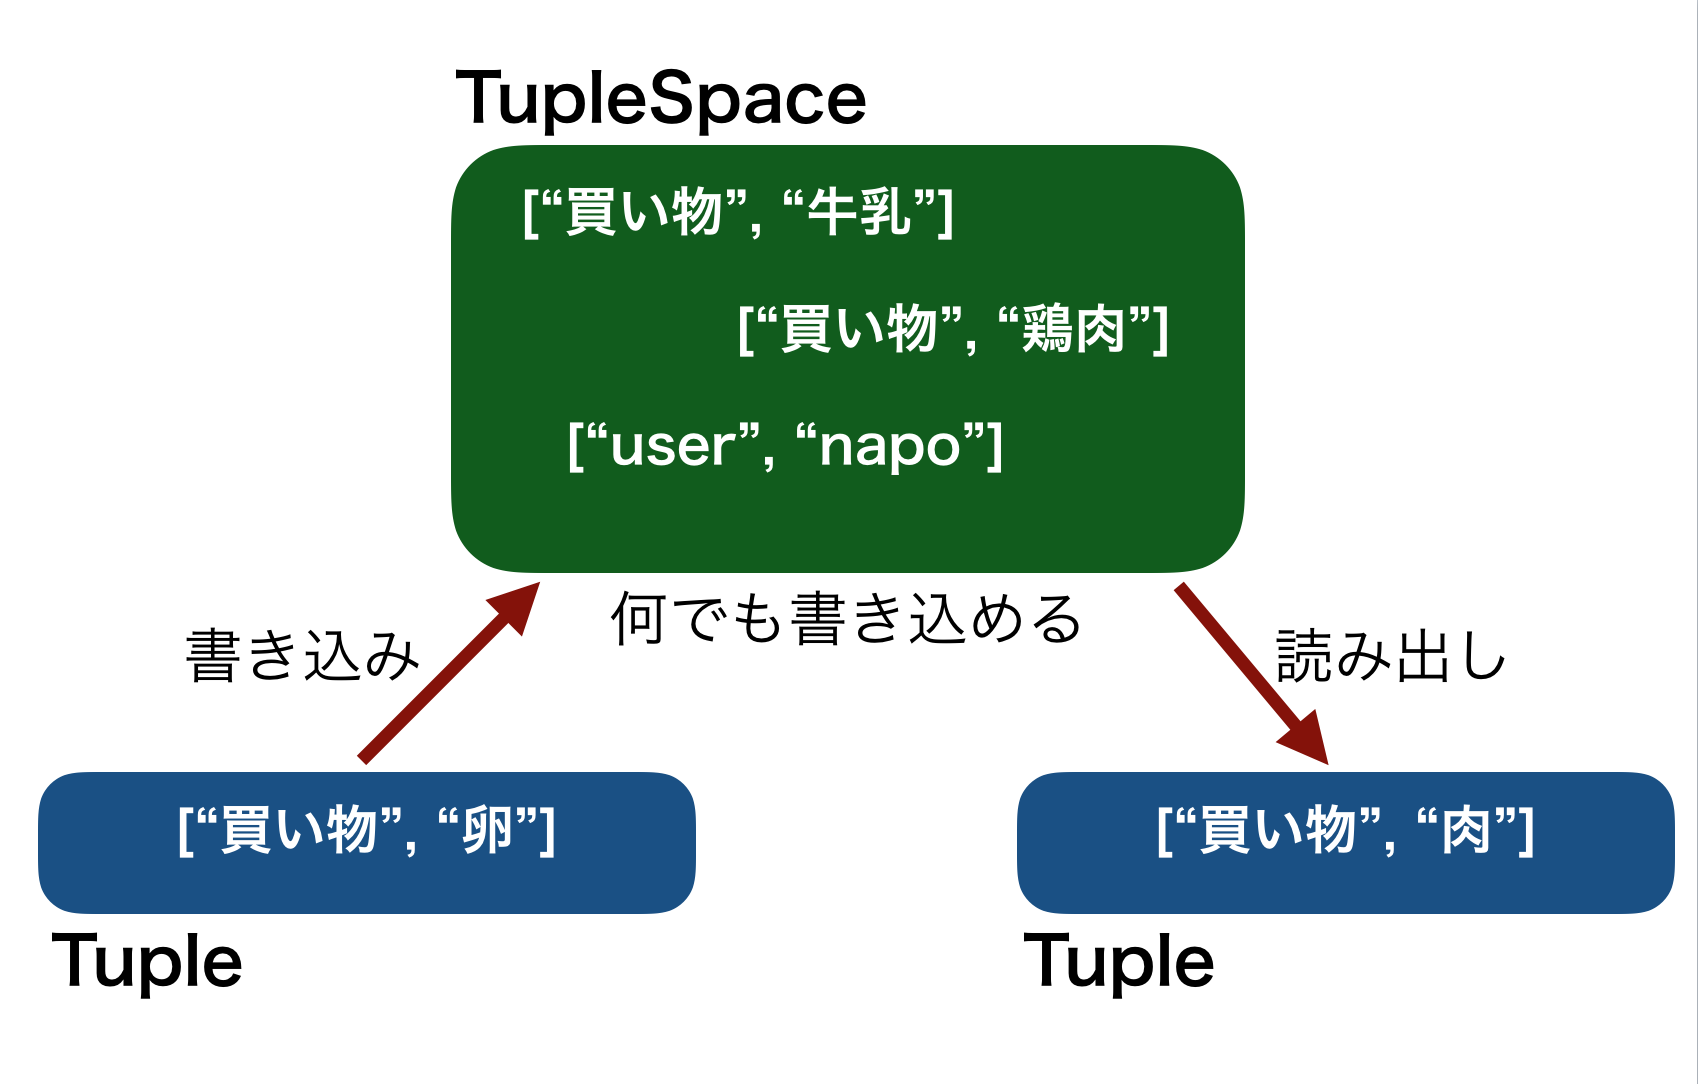
\includegraphics[width=7cm]{images/linda.png}
}
\caption{Linda}
\label{button}
\end{figure}

\subsection{WebLinda}
WebLindaは、橋本翔\footnote{http://shokai.org}氏が開発したオープンソースソフトウェアで、Node.js\footnote{https://nodejs.org}のWebSocketライブラリSocket.IO\footnote{http://socket.io}上に実装されたLindaシステムである。
通常のWebサーバ上に実装されているため、HTTP通信ができればWebLindaを使うことができる。
WebLindaは、\url{write, read, take, watch}の4つの基本操作によってプロセス間通信を行う。

\paragraph*{write}
新しいデータオブジェクト(タプル)を生成し共有空間(タプルスペース)に書き込む。

\vspace{2mm}
\paragraph*{read}
指定した形式に部分一致するタプルがタプルスペースにあるかどうか調べて1つ読み出す。
一致するものが無い場合は一致するタプルが書き込まれるまで待つ。

\vspace{2mm}
\paragraph*{take}
\url{read}しつつ、読み出したタプルをタプルスペースから削除する。

\vspace{2mm}
\paragraph*{watch}
タプルスペースを監視し、一致するタプルが\url{write}された瞬間に読み出す。

\subsection{『わかるらんど』でのWebLinda実装}
『わかるらんど』でのWebLinda実装について述べる。
ユーザのリアクションを表示する際には、
\begin{verbatim}
{
    from: "@napo0703",
    display: 60,
    value: "なる ほど",
    type: "reaction"
}
\end{verbatim}
というタプルをやりとりしている。
